\documentclass[12pt]{article}

\usepackage{amsmath,amssymb,amsthm,amscd,amsfonts}

\usepackage{tikz}

\usepackage{url}

\usepackage{fullpage}

\usepackage{mathtools}

\usepackage{rotating}

\DeclarePairedDelimiter\abs{\lvert}{\rvert}
\DeclarePairedDelimiter\paren{\lparen}{\rparen}

\def\subw{\mathrel{\triangleleft}}
\DeclareMathOperator\supe{sup}
\DeclareMathOperator\subb{sub}

\theoremstyle{plain}
\newtheorem{theorem}{Theorem}
\newtheorem{corollary}[theorem]{Corollary}
\newtheorem{lemma}[theorem]{Lemma}
\newtheorem{proposition}[theorem]{Proposition}
%\newtheorem{test}{Test}

\theoremstyle{definition}
\newtheorem{definition}[theorem]{Definition}
\newtheorem{example}[theorem]{Example}
\newtheorem{conjecture}[theorem]{Conjecture}

\theoremstyle{remark}
\newtheorem{remark}[theorem]{Remark}
\newtheorem{problem}[theorem]{Problem}

\newcommand{\0}{\mathtt{0}}
\newcommand{\1}{\mathtt{1}}
\newcommand{\2}{\mathtt{2}}
\newcommand{\3}{\mathtt{3}}
\newcommand{\4}{\mathtt{4}}
\newcommand{\5}{\mathtt{5}}
\newcommand{\6}{\mathtt{6}}
\newcommand{\7}{\mathtt{7}}
\newcommand{\8}{\mathtt{8}}
\newcommand{\9}{\mathtt{9}}
\newcommand{\A}{\mathtt{A}}
\newcommand{\B}{\mathtt{B}}
\newcommand{\union}{\cup}
\newcommand{\set}[2]{\{\,#1{}:{}#2\,\}}

\title{Minimal Elements for the Prime Numbers}

\author{Curtis Bright\\
School of Computer Science\\
University of Waterloo\\
Waterloo, ON  N2L 3G1\\
Canada\\
{\tt cbright@uwaterloo.ca} \\
\ \\
Raymond Devillers\\
D\'epartement d'Informatique, CP 212\\
Universit\'e Libre de Bruxelles \\
B-1050 Bruxelles\\
Belgium\\
{\tt rdevil@ulb.ac.be} \\
\ \\
Jeffrey Shallit \\
School of Computer Science\\
University of Waterloo\\
Waterloo, ON  N2L 3G1\\
Canada \\
{\tt shallit@cs.uwaterloo.ca}}

\begin{document}

\maketitle

\begin{abstract}
We say a string of symbols $s$ is {\it minimal} for a language $L$
if $s$ is a member of $L$, and it is not possible to obtain another 
member of $L$ by striking out one or more symbols from $s$.  Although
the set $M(L)$ of minimal strings is necessarily finite, determining
it explicitly for a given $L$ can be a difficult computational problem.  
We use some number-theoretic heuristics to compute $M(L)$, where $L$
is the language of base-$b$ representations of the prime numbers,
for $2 \leq b \leq 28$.
\end{abstract}

\section{Introduction}

Problems about the digits of prime numbers have a long history, and many
of them are still unsolved.  For example, are there infinitely many
primes, all of whose base-$10$ digits are $1$?  Currently,
there are only five
known, corresponding to $(10^p-1)/9$ for $p := 2$, $19$, $23$, $317$, and
$1031$.  It seems likely that four more are given by
$p := 49081$, $86453$, $109297$, and $270343$, but this has not yet been
rigorously proven.

Another problem on the digits of primes was introduced by the
third author \cite{Sh00}.  To describe it, we need some definitions.
We say that a string $x$ is a {\it subword} of a string $y$, and 
we write $x \subw y$, if 
one can strike out zero or more symbols of $y$ to get $x$.
For example, {\tt string} is a subword of
{\tt Meistersinger}.  
(In the literature, this concept is sometimes called a ``scattered
subword'' or ``substring''.)
A {\it language} is a set of strings.  A string $s$ is {\it minimal}
for $L$ if  (a) $s \in L$ and (b) if $x \in L$ and $x \subw s$, then
$x = s$.    The set of all minimal strings of $L$ is denoted $M(L)$.

In this paper, we describe a heuristic
technique for determining $M(L_b)$ in the
case where $L_b$ consists of the representations, in base $b$, of the
the prime numbers $\lbrace 2, 3, 5, \dotsc \rbrace$.  We obtain
a complete characterization of $M(L_b)$ for bases
$2 \leq b \leq 16$ and $b = 18,20,22,24$.   For the remaining
bases $b = 17,19,21,23,25,26,27,28$,
we obtain
results that allow us to ``almost'' completely characterize this set.

In what follows, if $x$ is a string of symbols over the alphabet
$\Sigma_b := \lbrace \0, \1, \dotsc, b-1 \rbrace$ we let 
$[x]_b$ denote the evaluation of $x$ in base $b$ (starting with the
most significant digit).  This is extended to languages as follows:
$[L]_b := \set{ [x]_b }{ x \in L }$.
We use the convention that $\A = 10$, $\B = 11$, and so forth,
to conveniently represent strings of symbols in base $b > 10$.
We let $(x)_b$ be the canonical representation
of $x$ in base-$b$, that is, the representation without leading zeroes.
%The set of all canonical representations in base $b$ is denoted
%$C_b$.
Finally, as usual, for a language $L$ we let
$L^n := \underbrace{LL\dotsm L}_n$ and $L^* := \bigcup_{i \geq 0} L^i$.

\section{Why minimal sets are interesting}

One reason why
the minimal set $M(L)$ of a language $L$ is interesting is because it
allows us to compute two natural and related languages,
defined as follows:
\begin{align*}
\subb(L) &:= \set{x \in \Sigma^*}{\text{there exists $y \in L$ such that $x \subw y$}} ; \\
\supe(L) &:= \set{x \in \Sigma^*}{\text{there exists $y \in L$ such that $y \subw x$}} .
\end{align*}

An amazing fact is that $\subb(L)$ and $\supe(L)$ are always regular.
This follows from
the following classical theorem due to Higman \cite{Hi52} and
Haines \cite{Ha69}.

\begin{theorem}
For every language $L$, there are only finitely many minimal strings.
\end{theorem}

Indeed, we have $\supe(L) = \supe(M(L))$
and $\Sigma^* - \subb(L) = \supe(M(\Sigma^* - \subb(L)))$, and
the superword language of a finite language is regular, since
\[ \supe\paren[\big]{\{w_1,\dotsc,w_n\}} = \bigcup_{i=1}^n \Sigma^* w_{i,1} \Sigma^* \dotsm \Sigma^* w_{i,\abs{w_i}} \Sigma^* \]
where $w_i=w_{i,1}\dotsm w_{i,\abs{w_i}}$ with $w_{i,j}\in\Sigma$.

\section{Why the problem is hard}

Determining $M(L)$ for arbitrary $L$
is in general unsolvable, and can be difficult even when $L$
is relatively simple~\cite{GHK07}.

The following is a ``semi-algorithm'' that 
is guaranteed to produce $M(L)$, but it is not so easy to implement:

\bigskip
\noindent (1) $ M := \emptyset$ \\
\noindent (2) while ($L \not= \emptyset$) do \\
\hphantom{} \qquad (3) choose $x$, a shortest string in $L$ \\
\hphantom{} \qquad (4) $ M := M \union \lbrace  x \rbrace$ \\
\hphantom{} \qquad (5) $ L := L - \supe(\lbrace x \rbrace) $ \\

\smallskip

In practice, for arbitrary $L$,
we cannot feasibly carry out step (5).  Instead, we work
with $L'$, some regular overapproximation to $L$, until we can show $L' =
\emptyset$ (which implies $L = \emptyset$).  In practice,
$L'$ is usually chosen to be a finite union of sets of the form 
$L_1 L_2^* L_3$, where each of $L_1$, $L_2$, $L_3$ is finite.
In the case we consider in this paper,
we then have to determine whether such a language contains
a prime or not.

However, it is not even known if the following simpler decision problem is 
recursively solvable:

\medskip

\begin{problem}
Given strings $x, y, z$, and a base $b$, does there exist a prime
number whose base-$b$ expansion is of the form $x \underbrace{yy\cdots y}_n z$
for some $n \geq 0$?
\end{problem}

\medskip

An algorithm to solve this problem, for example, would allow us to decide
if there are any additional Fermat primes (of the form $2^{2^n}+1$)
other than the known ones (corresponding to $n = 0$, $1$, $2$, $3$, $4$).

Therefore, in practice, we are forced to try to rule out prime
representations based on modular techniques and factorizations.
This is discussed in the next section.

\section{Some useful lemmas}\label{seclemmas}
It will be necessary for our algorithm to determine if families of the
form $[xL^*z]_b$ contain a prime or not.  We use two different strategies
to show that such families contain no primes.

In the first strategy, we mimic the well-known technique of ``covering
congruences'' \cite{Choi},
by finding some finite set $S$ of integers $N > 1$ such that
every number in a given family is divisible by some element of $S$.
In the second strategy, we attempt to find a
difference-of-squares or difference-of-cubes factorization.

\subsection{The first strategy}

We start with the simplest version of the idea:  to find 
an $N > 1$ that divides each element of the family $[xL^*z]_b$.
At first glance, this would require
checking that $N$ divides $xL^nz$ for $n=0$, $1$, $2$, $\dotsc$.
However, the following lemma shows that it is only necessary to check
the two cases $n=0$ and $1$.  Although divisibility based on digital
considerations has a long history (e.g., \cite[Chap.~XII]{Dick}),
we could not find these kinds of results in the literature.

\begin{lemma}\label{lemone}
Let $x$, $z\in \Sigma^*_b$, and let $L\subseteq\Sigma^*_b$.
Then 
$N$ divides all numbers of the form $[xL^*z]_b$
if and only if 
$N$ divides $[xz]_b$ and all numbers of the form $[xLz]_b$.
\end{lemma}
\begin{proof}%($\Rightarrow$)
Let $y=y_1\dotsm y_n\in L^*$, where $y_1$, $\dotsc$, $y_n\in L$.  
By telescoping we have
\[ [xyz]_b - [xz]_b = \sum_{i=1}^{n}([xy_{i}y_{i+1}\dotsm y_n z]_b-[xy_{i+1}\dotsm y_n z]_b) . \]
Cancelling the final $\abs{y_{i+1}\dotsm y_nz}$ base-$b$ digits in the summand difference ---
which are identical --- this becomes
\[ [xyz]_b = [xz]_b + \sum_{i=1}^{n}b^{\lvert{y_{i+1}\dotsm y_n z}\rvert}([xy_i]_b-[x]_b) . \]
But $b^{\lvert z\rvert}([xy_i]_b-[x]_b)=[xy_iz]_b-[xz]_b$ by 
adding and subtracting $[z]_b$, so we have
\[ [xyz]_b = [xz]_b + \sum_{i=1}^{n}b^{\vert{y_{i+1}\dotsm y_n}\rvert}([xy_iz]_b-[xz]_b) . \]
Since $N\mid[xz]_b$ and $N\mid[xy_iz]_b$ for each $1\leq i\leq n$,
 it follows that $N\mid[xyz]_b$.
 
The other direction is clear, since $[xz]_b$ and numbers of the 
form $[xLz]_b$ are both of the form $[xL^*z]_b$.
\end{proof}

In practice, our algorithm employs this lemma with 
$L:=\{y_1,\dotsc,y_n\}\subseteq\Sigma_b$, and all numbers of the form
$[xL^*z]_b$ are shown to be composite with the following corollary.
\begin{corollary}\label{corone}
If $1<\gcd([xz]_b,[xy_1z]_b,\dotsc,[xy_nz]_b)<[xz]_b$
 then all numbers of the form $[x\{y_1,\dotsc,y_n\}^*z]_b$ are composite.
\end{corollary}
\begin{proof}
By Lemma~\ref{lemone}, we know
that $N:=\gcd([xz]_b,[xy_1z]_b,\dotsc,[xy_nz]_b)>1$ 
divides all numbers of the form $[x\{y_1,\dotsc,y_n\}^*z]_b$.
By the size condition $N$ is strictly less than each such number, and
so is a nontrivial divisor.
\end{proof}

\begin{example}
Since $\gcd(49, 469)=7$, every number with base-$10$ representation
of the form $\4\6^*\9$ is 
divisible by $7$.
Since $1 < 7 < 49$, each such number is composite.
\end{example}

We also generalize this to the following corollary in the case where 
a single divisor does not divide each number in the family.
\begin{corollary}\label{cortwo}
Let $L := \lbrace y_1, y_2, \ldots, y_n \rbrace$.
If \[N_0:=\gcd \paren[\big]{ \{ [xz]_b \} \union [xL^2 z]_b} \]
and
\[ N_1:= \gcd \paren[\big]{[xLz]_b \union [xL^3z]_b} \]
lie strictly between $1$ and $[xz]_b$, then all numbers of the form 
$[xL^*z]_b$ are composite.
\end{corollary}
\begin{proof}
By Lemma~\ref{lemone} applied
to $[x(L^2)^*z]_b$, we know that $N_0$ divides all numbers of the 
form $[x L^* z]_b$ in which an even number of $y_i$ appear.
By Lemma~\ref{lemone} on $[xy_i(L^2)^*z]_b$ 
for each $1\leq i\leq n$, we know that $N_1$ 
divides all numbers of the form $[x L^* z]_b$ for which an 
odd number of $y_i$ appear.
By the size conditions, $N_0$ and $N_1$ are nontrivial divisors.
\end{proof}

\begin{example}
Since $\gcd([\6]_9,[\6\1\1]_9)=2$, every number with
base-$9$ representation of the form $\6\1^*$ of 
odd length is divisible by $2$.
Since $\gcd([\6\1]_9,[\6\1\1\1]_9)=5$,
every number with base-$9$ representation of the form $\6\1^*$ 
of even length is divisible by $5$.  Since these numbers lie 
strictly between $1$ and $6$, every number with base-$9$
representation of the form $\6\1^*$ is 
composite.
\end{example}

We also note that it is simple to generalize Corollary~\ref{cortwo}
to apply to 
check if there are divisors $N_0$, $N_1$, $\dotsc$, $N_{k-1}$ such that
$N_i$ divides all numbers of the form $[x\{y_1,\dotsc,y_n\}^*z]_b$ in which 
the number of $y_i$ appearing is congruent to $i\bmod k$.
\begin{example}
Let $b := 16$.
Then
$7$ divides $[\8\A\0\1]_b$ and $[\8\A\0\A\A\A\1]_b$.
Furthermore, $13$ divides 
$[\8\A\0\A\1]_b$ and $[\8\A\0\A\A\A\A\1]_b$,
and $3$ divides $[\8\A\0\A\A\1]_b$ and 
$[\8\A\0\A\A\A\A\A\1]_b$.  Thus all numbers with base-$16$
representation of the form $\8\A\0\A^*\1$ are 
divisible by either $7$, $13$, or $3$, depending on their 
length mod $3$.
\end{example}

A version of Lemma~\ref{lemone} which applies to the most general kind 
of family we need to consider ($x_1L_1^*\dotsm x_mL_m^*$)
is formulated in Lemma~\ref{lemtwo}.

\begin{lemma}\label{lemtwo}
Let $x_1$, $\dotsc$, $x_m\in \Sigma^*_b$, and $L_1$, $\dotsc$, 
$L_m\subseteq\Sigma^*_b$.  Then
$N$ divides all numbers of the form $[x_1L_1^*x_2L_2^*\dotsm x_mL_m^*]_b$
if and only if
$N$ divides $[x_1\dotsm x_m]_b$ and all numbers of the form 
$[x_1L_1x_2x_3\dotsm x_m]_b$, $\dotsc$, $[x_1\dotsm x_{m-1}x_mL_m]_b$.
\end{lemma}
\begin{proof}
Say $w\in x_1L_1^*x_2L_2^*\dotsm x_mL_m^*$; then there exist
$y_{i,1}$, $\dotsc$, $y_{i,n_i}\in L_i$ such that
\[ w = x_1y_{1,1}\dotsm y_{1,n_1}x_2y_{2,1}\dotsm y_{2,n_2}\dotsm x_m y_{m,1}\dotsm y_{m,n_m} \]
for $1\leq i\leq m$.
As in the proof of Lemma~\ref{lemone}, we have that
\[ [w]_b = [x_1\dotsm x_m]_b + \sum_{i=1}^m\sum_{j=1}^{n_i} b^{\abs{y_{i,j+1}\dotsm y_{m,n_m}}}([x_1\dotsm x_i y_{i,j} x_{i+1}\dotsm x_m]_b-[x_1\dotsm x_m]_b) \]
from which the claim follows.
\end{proof}
As in Lemma~\ref{lemone}, we typically apply this lemma in the case 
where each $L_i\subseteq\Sigma_b$ and show that all numbers of the 
form $[x_1L_1^*x_2L_2^*\dotsm x_mL_m^*]_b$ have a divisor.
\begin{example}
Take $(L_1, L_2, L_3) := (\{ \0 \},\{\0\},\emptyset)$ and $(x_1,x_2, x_3) := (\9, \8, \1)$.
Since $9$ divides $981$, $9081$, and $9801$, it follows that $9$ 
divides every number with base-$10$ representation
of the form $\9\0^*\8\0^*\1$.
\end{example}

More generally, if a single divisor doesn't work for every number, 
Lemma~\ref{lemtwo} can also be applied in the case where all numbers 
of the form $[x_1L_1^*\dotsm x_i(L_i^2)^*\dotsm x_mL_m^*]_b$ have one
divisor, and all numbers of the form 
$[x_1L_1^*\dotsm x_iL_i(L_i^2)^*\dotsm x_mL_m^*]_b$ have another divisor.
\begin{example}
Let $b := 11$.
Since $3$ divides each of $[\4\4\A\1]_b$,
$[\4\4\A\1\1\1]_b$,
$[\4\4\0\A\1]_b$ ,
it follows that
every number of the form $[\4\4\0^*(\1\1)^*\1]_b$ is composite.
Since $2$ divides each of $[\4\4\A\1\1]_b$,
$[\4\4\A\1\1\1\1]_b$, $[\4\4\0\A\1\1]_b$, we know
every number of the form $[\4\4\0^*(\1\1)^*\1\1]_b$ is composite.
It follows that all numbers of the form $[\4\4\0^*\A\1^*\1]_b$ are composite.
\end{example}

Lemma~\ref{lemtwo} can also be applied to the case when all even-length 
strings under consideration have one divisor, and all the odd-length 
strings have another divisor.  One such case is, for example,
if numbers of the form 
$[x_1(L_1^2)^*x_2(L_2^2)^*x_3]_b$ and $[x_1 L_1(L_1^2)^*x_2L_2(L_2^2)^*x_3]_b$ 
have one divisor, and numbers of the form $[x_1L_1(L_1^2)^*x_2(L_2^2)^*x_3]_b$ 
and $[x_1(L_1^2)^*x_2L_2(L_2^2)^*x_3]_b$ have another divisor.
\begin{example}
Let $b := 9$.
Since $2$ divides each of $[\6]_b$,
$[\1\1\6]_b$,
$[\6\1\1]_b$,
$[\1\6\1]_b$,
$[\1\1\1\6\1]_b$, 
$[\1\6\1\1\1]_b$, every odd-length string of the form $\1^*\6\1^*$ is 
composite.
Since $5$ divides each of $[\1\6]_b$,
$[\1\1\1\6]_b$,
$[\1\6\1\1]_b$,
$[\6\1]_b$,
$[\1\1\6\1]_b$, 
$[\6\1\1\1]_b$,
every even-length string of the form $\1^*\6\1^*$ is composite.
\end{example}

\subsection{The second strategy}

A second way of proving that families of the form $xL^*z$ do not contain a 
prime is via algebraic factorizations, such as a difference-of-squares 
factorization.

\begin{lemma}\label{lemsquares}
Let $x$, $y$, $z\in\Sigma^*_b$, and let $g:=\gcd([y]_b,b-1)$, 
$X:=([y]_b+(b-1)[x]_b)/g$, and $Y:=(b^{\lvert{z}\rvert}[y]_b-(b-1)[z]_b)/g$.
If\/ $b$, $X$, and $Y$ are all squares and 
$\sqrt{b^{\lvert z\rvert}X}-\sqrt{Y}>(b-1)/g$, then all numbers of the form
 $[xy^*z]_b$ are composite.
\end{lemma}
\begin{proof}
Evaluating the base-$b$ expansion of $xy^nz$, we get
\begin{align*}
[xy^nz]_b &= b^{\lvert z\rvert+n}[x]_b + b^{\lvert z\rvert}\frac{b^n-1}{b-1}[y]_b + [z]_b \\
&= \frac{b^{\lvert z\rvert+n}X-Y}{(b-1)/g} . 
%= \frac{(\sqrt{Xb^{\lvert z\rvert+n}}+\sqrt{Y})(\sqrt{Xb^{\lvert z\rvert+n}}-\sqrt{Y})}{(b-1)/g}
\end{align*}
Since $b$, $X$, and $Y$ are all squares the numerator factors as a 
difference of squares.  By the size condition both factors are 
strictly larger than the
denominator, and so the factorization is nontrivial.
\end{proof}

\begin{example}
Let $b:=16$, $x:=\4$, $y:=\4$, and $z:=\1$.  Then $g=1$, $X=8^2$, $Y=7^2$, and
\[ [\4\4^n\1]_b = \frac{(4^{n+1}\cdot8+7)(4^{n+1}\cdot8-7)}{15} . \]
Since $4\cdot8-7>15$, this factorization is nontrivial and no number of 
the form $[\4\4^*\1]_b$ is prime.
\end{example}

It is also possible to combine Lemma~\ref{lemtwo} with Corollary~\ref{cortwo} 
to construct a test which also applies to bases which are not squares.
\begin{corollary}
Using the same setup as in Lemma~\ref{lemtwo}, if\/ $b^{\abs{z}}X$ and $Y$ 
are squares, $\sqrt{b^{\lvert z\rvert}X}-\sqrt{Y}>(b-1)/g$, and
$1<\gcd([xyz]_b,[xy^3z]_b)<[xz]_b$, then all numbers of the form $[xy^*z]_b$ 
are composite.
\end{corollary}
\begin{proof}
Say $n=2m$ is even.  Then from the factorization in Lemma~\ref{lemtwo},
\[ [xy^nz]_b = \frac{(b^m\sqrt{b^{\abs{z}}X}+\sqrt{Y})(b^m\sqrt{b^{\abs{z}}X}-\sqrt{Y})}{(b-1)/g} \]
which is nontrivial by the size condition.

Alternatively, if $n$ is odd then as in Corollary~\ref{cortwo} we have that 
$\gcd([xyz]_b,[xy^3z]_b)$ divides $[xy^nz]_b$, and by the size condition this 
divisor is nontrivial.
\end{proof}
\begin{example}
Let $b:=17$, $x:=\1\9$, $y:=\9$, and $z:=\9$.  Then $g=1$, 
$b^{\abs{z}}X=85^2$, $Y=3^2$, and
\[ [xy^{2n}z]_b = \frac{(17^n\cdot85+3)(17^n\cdot85-3)}{16} . \]
Since $85-3>16$ this factorization is nontrivial.  Furthermore, all numbers 
of the form $[xy^{2n+1}z]_b$ are even, so all numbers of the form 
$[\1\9\9^*\9]_b$ are composite.
\end{example}
Finally, we present a variant of Lemma~\ref{lemsquares} which applies to a 
difference-of-cubes factorization.
\begin{lemma}\label{lemcubes}
Let $x$, $y$, $z\in\Sigma^*_b$, and let $g:=\gcd([y]_b,b-1)$, 
$X:=([y]_b+(b-1)[x]_b)/g$, and $Y:=(b^{\lvert{z}\rvert}[y]_b-(b-1)[z]_b)/g$.
If\/ $b$, $X$, and $Y$ are all cubes and 
$\sqrt[3]{b^{\lvert z\rvert}X}-\sqrt[3]{Y}>(b-1)/g$, then all numbers of 
the form
 $[xy^*z]_b$ are composite.
\end{lemma}
\begin{proof}
As in Lemma~\ref{lemsquares}, we have
\[ [xy^nz]_b = \frac{\bigl((b^{\abs{z}+n}X)^{1/3}-Y^{1/3}\bigr)\bigl((b^{\abs{z}+n}X)^{2/3}+(b^{\abs{z}+n}XY)^{1/3}+Y^{2/3}\bigr)}{(b-1)/g} . \]
The second factor is at least as large as the first (except in the 
single case $b^{\abs{z}+n}X=1$ and $Y=-1$, which is not possible by 
construction of $X$ and~$Y$),
so by the size condition both factors are strictly larger than the 
denominator, and the factorization is nontrivial.
\end{proof}
\begin{example}
Let $b:=8$, $x:=\1$, $y:=\0$, and $z:=\1$.  Then $g=7$, $X=1$, $Y=-1$, and
\[ [\1\0^n\1]_b = (2^{n+1}+1)(4^{n+1}-2^{n+1}+1) . \]
Since $2-(-1)>1$, this factorization is nontrivial and no number of the 
form $[\1\0^*\1]_b$ is prime.
\end{example}

\section{Our heuristic algorithm}

As previously mentioned, in practice to compute $M(L_b)$ one works with an underapproximation
$M$ of $M(L_b)$ and an overapproximation $L$ of $L_b-\sup(M)$.
One then refines such approximations until $L=\emptyset$ from which it follows that $M=M(L_b)$.

For the initial approximation, note that every minimal prime in base $b$ with at least 4
digits is of the form $x Y^* z$, where $x\in\Sigma_b-\{\0\}$, $z\in\Sigma_b$, and
\[ Y := \Sigma_b - \set{y}{\text{$(p)_b\subw xyz$ for some prime $p$}} . \]
Making use of this, our algorithm sets $M$ to be the set of base-$b$ representations
of the minimal primes with at most $3$ digits (which can be found simply by brute force)
and $L$ to be $\bigcup_{x,z}xY^*z$, as described above.

All remaining minimal primes are members of $L$, so to find them we explore the families in~$L$.
During this process, each family will be decomposed into possibly multiple other families.
For example, a simple way of exploring the family $xY^*z$ where $Y:=\{y_1,\dotsc,y_n\}$ is to decompose it
into the families $xY^*y_1z$, $\dotsc$, $xY^*y_nz$.  If the smallest member (say $xy_iz$)
of any such family happens to be prime, it can be added to $M$ and the family
$xY^*y_iz$ removed from consideration.  Furthermore, once $M$ has been updated it may be possible
to simplify some families in $L$.  In this case, $xY^*y_jz$ (for $j\neq i$) can be simplified to
$x(Y-\{y_i\})^*y_jz$ since no minimal prime contains $xy_iz$ as a proper subword.

Another way of decomposing %families 
the family $xY^*z$ is possible if one knows that a digit of $Y$ can only occur a certain number
of times.  For example, if $xy_iy_iz$ has a proper prime subword then the digit $y_i$
can occur at most once in any minimal prime of the form $xY^*z$, and we can split $xY^*z$ into
the two families
\[ x(Y-\{y_i\})^*z \qquad\text{and}\qquad x(Y-\{y_i\})^*y_i(Y-\{y_i\})^*z .\]

Lastly, the family $xY^*z$ can be decomposed by considering digits of $Y$ which are mutually incompatible,
i.e., they cannot occur simultaneously in a minimal prime.  For example, if $xy_iy_jz$ and $xy_jy_iz$ ($i\neq j$)
both have proper prime subwords then the digits $y_i$ and $y_j$ cannot occur simultaneously in any minimal
prime of the form $xY^*z$, and we can split $xY^*z$ into the two families
\[ x(Y-\{y_i\})^*z \qquad\text{and}\qquad x(Y-\{y_j\})^*z . \]
Sometimes it is not possible to show two digits are mutually incompatible, but it is possible to know that
one digit must appear before the other.  For example, if $xy_iy_jz$ has a proper prime subword then the digit
$y_j$ must appear before $y_i$ in any minimal prime of the form $xY^*z$, and we can replace $xY^*z$
with the family
\[ x(Y-\{y_i\})^*(Y-\{y_j\})^*z . \]
Similarly, if $xy_jyy_iz$ has a proper prime subword then we can split $xY^*yY^*z$ into the two families
\[ x(Y-\{y_i\})^*yY^*z \qquad\text{and}\qquad xY^*y(Y-\{y_j\})^*z . \]

We now formulate these arguments for the most general kind of family we need to consider, namely
$x_1L_1^*\dotsm x_mL_m^*$.  For simplicity, we only specify the decompositions as applying to
$L_1:=\{y_1,\dotsc,y_n\}$, but it is straightforward to generalize these decompositions
to also apply to $L_i$ for any $1\leq i\leq m$.

\begin{lemma}\label{lemexplore}
Every minimal prime of the form $x_1L_1^*\dotsm x_mL_m^*$ must also be of the form
$x_1x_2L_2^*\dotsm x_mL_m^*$ or $x_1y_iL_1^*x_2L_2^*\dotsm x_mL_m^*$ for some $1\leq i\leq n$.
\end{lemma}
\begin{proof}
Follows from the fact that $L_1^*=\{\epsilon\}\cup\bigcup_{i=1}^n y_iL_1^*$.
\end{proof}
Similarly, one can generalize Lemma~\ref{lemexplore} to apply to adding characters to the right of $L_1$ rather than
to the left.
\begin{example}
The family $\1\0\{\0,\1\}^*\6\1^*\1$ splits into the three families $\1\0\6\1^*\1$, $\1\0\{\0,\1\}^*\0\6\1^*\1$, and $\1\0\{\0,\1\}^*\1\6\1^*\1$
by exploring $\{\0,\1\}^*$ on the right.
\end{example}

\begin{lemma}\label{lemsplit1}
If $x_1y_i^kx_2\dotsm x_m$ contains a prime proper subword (for some $k>0$) then every minimal prime of the form
$x_1L_1^*\dotsm x_mL_m^*$ is of the form \[x_1(L_1-\{y_i\})^*(y_i(L_1-\{y_i\})^*)^jx_2L_2^*\dotsm x_mL_m^*\]
for some $0\leq j<k$.
\end{lemma}
\begin{proof}
If $w\in x_1L_1^*\dotsm x_mL_m^*$ then $w\in x_1yx_2L_2^*\dotsm x_mL_m^*$ for some $y\in L_1^*$.
If $y$ contains $k$ or more instances of $y_i$ then by assumption it follows that $w$ contains a proper prime subword,
and therefore is not a minimal prime.  So if $w$ is a minimal prime then $y$ must contain less than $k$
instances of $y_i$, i.e., $y$ must be of the form $(L_1-\{y_i\})^*(y_i(L_1-\{y_i\})^*)^j$ for some $0\leq j<k$,
from which the claim follows.
\end{proof}
\begin{example}
The string $\6\6\1$ represents a prime in base 9, and is a proper subword of $\1\0\6\6\1$.  It follows that
the family $\1\0\{\0,\1,\6\}^*\1$ splits into the families
$\1\0\{\0,\1\}^*\1$ and $\1\0\{\0,\1\}^*\6\{\0,\1\}^*\1$ in base 9.
\end{example}

\begin{lemma}\label{lemsplit2}
If $x_1y_iy_jx_2\dotsm x_m$ and $x_1y_iy_jx_2\dotsm x_m$ contain prime proper subwords (where $i\neq j$) then 
every minimal prime of the form $x_1L_1^*\dotsm x_mL_m^*$ is of the form
\[x_1(L_1-\{y_i\})^*x_2L_2^*\dotsm x_mL_m^* \qquad\text{or}\qquad x_1(L_1-\{y_j\})^*x_2L_2^*\dotsm x_mL_m^* . \]
\end{lemma}
\begin{proof}
If $w\in x_1L_1^*\dotsm x_mL_m^*$ then $w\in x_1yx_2L_2^*\dotsm x_mL_m^*$ for some $y\in L_1^*$.
If $y$ contains both $y_i$ and $y_j$ then by assumption it follows that $w$ contains a proper prime subword,
and therefore is not a minimal prime.  So if $w$ is a minimal prime then $y$ cannot contain $y_i$ and $y_j$
simultaneously, i.e., $y$ must be of the form $(L-\{y_i\})^*$ or $(L-\{y_j\})^*$, from which the claim follows.
\end{proof}
\begin{example}
The string $\4\6\1\1$ represents a prime in base 8, and is a proper subword of $\4\4\6\4\1\1$ and $\4\4\4\6\1\1$.
It follows that the family $\4\4\{\4,\6\}^*\1\1$ splits into the families
$\4\4\4^*\1\1$ and $\4\4\6^*\1\1$ in base 8.
\end{example}

\begin{lemma}\label{lemsplit2b}
If $x_1y_iy_jx_2\dotsm x_m$ contains a prime proper subword (where $i\neq j$) then every minimal prime of the form
$x_1L_1^*\dotsm x_mL_m^*$ is of the form \[x_1(L_1-\{y_i\})^*(L_1-\{y_j\})^*x_2L_2^*\dotsm x_mL_m^* . \]
\end{lemma}
\begin{proof}
If $w\in x_1L_1^*\dotsm x_mL_m^*$ then $w\in x_1yx_2L_2^*\dotsm x_mL_m^*$ for some $y\in L_1^*$.
If $y$ contains $y_i$ before $y_j$ then by assumption it follows that $w$ contains a proper prime subword,
and therefore is not a minimal prime.  So if $w$ is a minimal prime then $y$ cannot contain $y_i$ before~$y_j$,
i.e., $y$ must be of the form $(L-\{y_i\})^*(L-\{y_j\})^*$, from which the claim follows.
\end{proof}
%\begin{example}
%The string $\1\0$ represents a prime in base 11, and is a proper subword of $\9\1\0\1$.
%It follows that the family $\9\{\0,\1\}^*\1$ splits into the family $\9\0^*\1^*\1$ in base 11.
%\end{example}
\begin{example}
The string $\1\0$ represents a prime in base 11, and is a proper subword of $\9\0\1\0\1$.
It follows that the family $\9\0\{\0,\1,\9\}^*\1$ splits into the family $\9\0\{\0,\9\}^*\{\1,\9\}^*\1$ in base 11.
\end{example}

\begin{lemma}\label{lemsplit2c}
If $x_1y_ix_2y_{2,j}x_3\dotsm x_m$ contains a prime proper subword (where $y_{2,j}\in L_2$) then every minimal prime of the form
$x_1L_1^*\dotsm x_mL_m^*$ is of the form
\[x_1(L_1-\{y_i\})^*x_2L_2^*\dotsm x_mL_m^* \qquad\text{or}\qquad x_1L_1x_2(L_2-\{y_{2,j}\})^*x_3L_3^*\dotsm x_mL_m^* . \]
\end{lemma}
\begin{proof}
If $w\in x_1L_1^*\dotsm x_mL_m^*$ then $w\in x_1yx_2y'x_3L_3^*\dotsm x_mL_m^*$ for some $y\in L_1^*$ and $y'\in L_2^*$.
If $y$ contains $y_i$ and $y'$ contains $y_{2,j}$ then by assumption it follows that $w$ contains a proper prime subword,
and therefore is not a minimal prime.  So if $w$ is a minimal prime then either $y$ cannot contain $y_i$ or $y'$ cannot
contain $y_{2,j}$, i.e., $y$ is of the form $(L_1-\{y_i\})^*$ and $y'$ is of the form $L_2^*$, or $y$ is of the form
$L_1^*$ and $y'$ is of the form $(L_2-\{y_{2,j}\})^*$, from which the claim follows.
\end{proof}
\begin{example}
The string $\6\0\4\1\1$ represents a prime in base 8, and is a proper subword of $\6\0\4\1\0\1$.
It follows that the family $\6\0\{\0,\4\}^*\1\0^*\1$ splits into the families
$\6\0\0^*\1\0^*\1$ and $\6\0\{\0,\4\}^*\1\1$ in base 8.
\end{example}

We call families of the form $xy^*z$ (where $x$, $z\in\Sigma_b^*$ and $y\in\Sigma_b$) \emph{simple} families.
Our algorithm then proceeds as follows:
\begin{enumerate}
\item $M:=\{\text{minimal primes in base $b$ of length $\leq3$}\}$ \\
$L:=\bigcup_{x,z\in\Sigma_b}xY^*z$, where $x\neq\0$ and $Y$ is the set of digits $y$ such that $xyz$ has no subword in $M$
\item While $L$ contains non-simple families:
\begin{enumerate}
\item Explore each family of $L$ by applying Lemma~\ref{lemexplore}, and update $L$.
\item Examine each family of $L$:
\begin{enumerate}
\item Let $w$ be the shortest string in the family.  If $w$ has a subword in $M$, then remove the family from $L$.
If $w$ represents a prime, then add $w$ to $M$ and remove the family from $L$.
\item If possible, simplify the family by applying Lemma~\ref{lemsplit1} with $k=1$.
\item Using the techniques of Section~\ref{seclemmas}, check if the family can be proven to only contain
composites, and if so then remove the family from $L$.
\end{enumerate}
\item Apply Lemmas~\ref{lemsplit1}, \ref{lemsplit2}, \ref{lemsplit2b}, and~\ref{lemsplit2c} to the families of $L$ as much
as possible and update $L$; after each split examine the new families as in~(b).
\end{enumerate}
\end{enumerate}

When exploring the families in line~(a), one should not always apply Lemma~\ref{lemexplore} directly as stated by adding
characters to the left of $L_1$; in our implementation we alternate (with period 4) between adding characters
to the left/right of the first/last nonempty $L_i$.  Also, the application of Lemma~\ref{lemsplit2b} tended to initially
produce an excess number of cases, so it was useful to only apply it following a certain number of iterations.  It also led to
duplicate families after simplifying, for example families of the form $xy^*y^ny^*z$ for varying $n$,
but these could be detected and removed.

The process of exploring/examining/splitting a family can be concisely expressed in a tree of decompositions.
A sample tree of decompositions, for the family $\1\{\0,\1,\6\}^*\1$ in base~9, is displayed in Figure~\ref{decomptree}.
When applying Lemma~\ref{lemexplore} on a family with only one nonempty $L_i$ we don't show the first decomposition
(simply removing $L_i^*$) since that results in the shortest word in the family, which is always implicitly
checked for primality/minimal subwords at each step anyway.

At the conclusion of the algorithm described, $L$ will consist of simple families (of the form $xy^*z$) which have not yet
yielded a prime, but for which there is no obvious reason why there can't be a prime of such a form.
In such a case, the only way to proceed is to test the primality of larger and larger numbers of such form and hope
a prime is eventually discovered.

The numbers in simple families are of the form $(ab^n+c)/d$ for some fixed $a$, $b$, $c$, $d$ where $d\mid ab^n+c$ for all $n$.
Except when $c=\pm1$ and $d=1$, it is too expensive to run a true primality test on such a number when $n$ is large.
In this case one must resort to a pseudoprimality test such as a Miller--Rabin test, unless a divisor of the number can be found.
Since we are testing many numbers in an exponential sequence, it is possible to use a sieving process to find divisors
rather than using trial division.

To do this, we made use of Geoffrey Reynolds' srsieve software~\cite{srsieve}.  This program uses the baby-step giant-step
algorithm to find all primes $p$ which divide $ab^n+c$ where $p$ and $n$ lie in a specified range.  Since this program cannot
handle the general case $(ab^n+c)/d$ when $d>1$ we only used it to sieve the sequence $ab^n+c$ for primes $p\nmid d$, and manually
removed those numbers for which $p\mid(ab^n+c)/d$.

After the numbers with small divisors had been removed, it remained to test the remaining numbers using a pseudoprimality test.
In the case $d=1$ we used the software LLR by Jean Penn\'e~\cite{llr}, and when $d>1$ we used custom software written using GMP~\cite{gmp}.
In the cases where the elements of $M(L_b)$ could be proven prime rigorously,
we employed PRIMO by Marcel Martin~\cite{primo}, an elliptic curve primality proving implementation.

\begin{sidewaysfigure}\begin{tiny}\[ 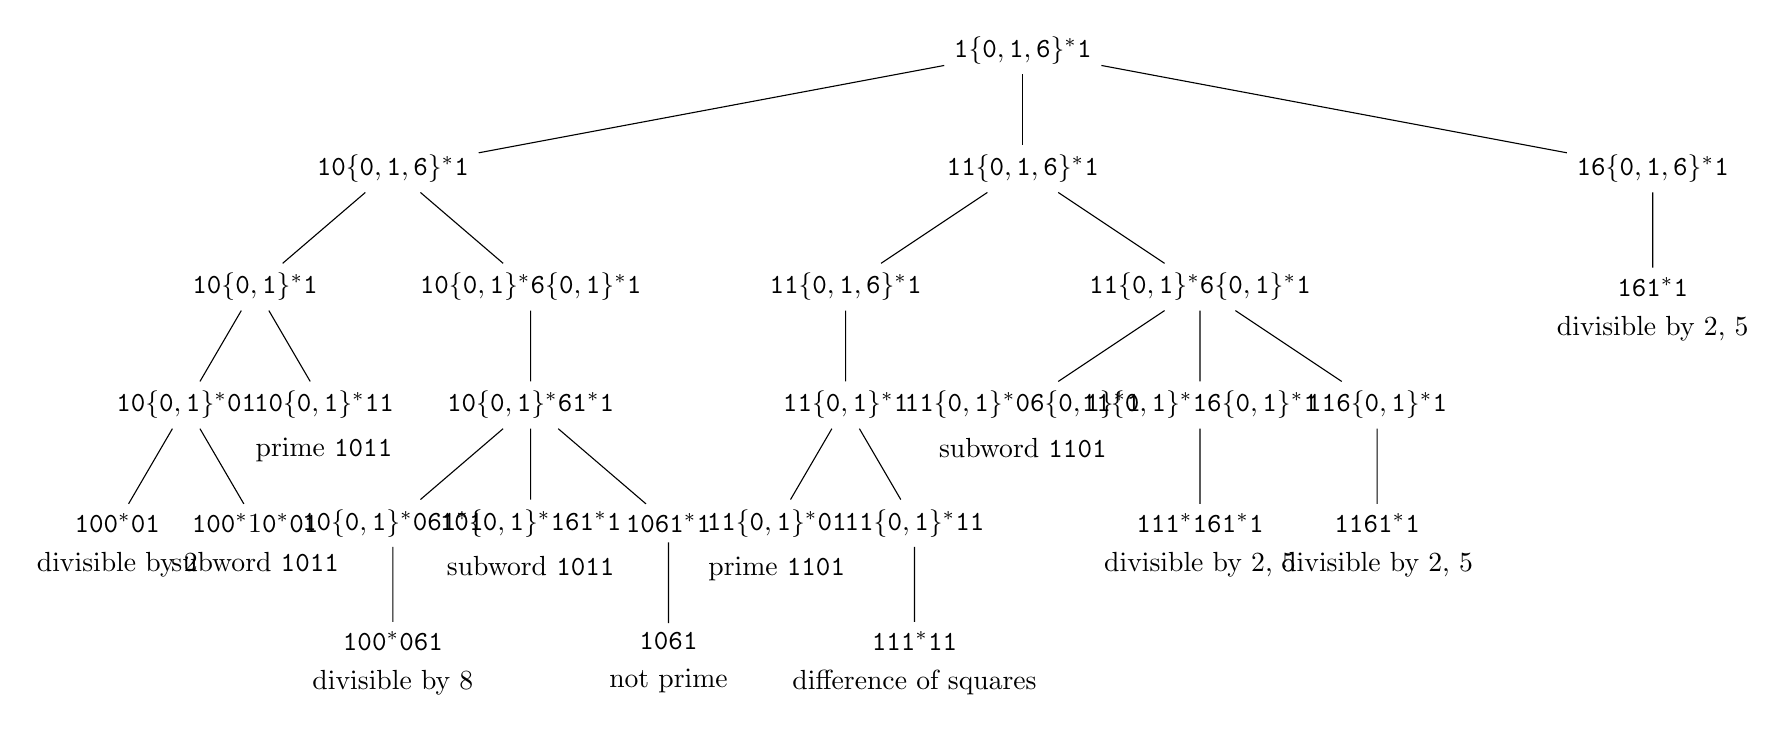
\begin{tikzpicture}
\node{$\1\{\0,\1,\6\}^*\1$}[sibling distance=8cm]
	child{node{$\1\0\{\0,\1,\6\}^*\1$}[sibling distance=3.5cm]
		child{node{$\1\0\{\0,\1\}^*\1$}[sibling distance=1.75cm]
			child{node{$\1\0\{\0,\1\}^*\0\1$}
				child{node[label=below:{divisible by 2}]{$\1\0\0^*\0\1$}}
				child{node[label=below:{subword $\1\0\1\1$}]{$\1\0\0^*1\0^*\0\1$}}}
			child{node[label=below:{prime $\1\0\1\1$}]{$\1\0\{\0,\1\}^*\1\1$}}}
		child{node{$\1\0\{\0,\1\}^*\6\{\0,\1\}^*\1$}[sibling distance=1.75cm]
			child{node{$\1\0\{\0,\1\}^*\6\1^*\1$}
				child{node{$\1\0\{\0,\1\}^*\0\6\1^*\1$}
					child{node[label=below:{divisible by 8}]{$\1\0\0^*\0\6\1$}}}
				child{node[label=below:{subword $\1\0\1\1$}]{$\1\0\{\0,\1\}^*\1\6\1^*\1$}}
				child{node{$\1\0\6\1^*\1$}
					child{node[label=below:{not prime}]{$\1\0\6\1$}}}}}}
	child{node{$\1\1\{\0,\1,\6\}^*\1$}[sibling distance=4.5cm]
		child{node{$\1\1\{\0,\1,\6\}^*\1$}[sibling distance=1.75cm]
			child{node{$\1\1\{\0,\1\}^*\1$}
				child{node[label=below:{prime $\1\1\0\1$}]{$\1\1\{\0,\1\}^*\0\1$}}
				child{node{$\1\1\{\0,\1\}^*\1\1$}
					child{node[label=below:{difference of squares}]{$\1\1\1^*\1\1$}}}}}
		child{node{$\1\1\{\0,\1\}^*\6\{\0,\1\}^*\1$}[sibling distance=2.25cm]
			child{node[label=below:{subword $\1\1\0\1$}]{$\1\1\{\0,\1\}^*\0\6\{\0,\1\}^*\1$}}
			child{node{$\1\1\{\0,\1\}^*\1\6\{\0,\1\}^*\1$}
				child{node[label=below:{divisible by 2, 5}]{$\1\1\1^*\1\6\1^*\1$}}}
			child{node{$\1\1\6\{\0,\1\}^*\1$}
				child{node[label=below:{divisible by 2, 5}]{$\1\1\6\1^*\1$}}}}}
	child{node{$\1\6\{\0,\1,\6\}^*\1$}[sibling distance=5cm]
		child{node[label=below:{divisible by 2, 5}]{$\1\6\1^*\1$}[sibling distance=3cm]}};
\end{tikzpicture} \]\end{tiny}\caption{Tree of decompositions for $\1\{\0,\1,\6\}^*\1$ in base $9$.}\label{decomptree}\end{sidewaysfigure}

\section{Results}
A summary of the results of our algorithm is presented in 
Figure~\ref{resultsfig}.
For each base $b$ between 2 and 16,
we give the size $|M(L_b)|$ and ``width'' $\max_{x \in M(L_b)} |x|$ of
the corresponding family.
For bases between 17 and 28 a lower bound on the size and width of
$M(L_b)$ is given, along with the number of families of the form
$xy^*z$ for which no prime member could be found, nor could the family be
ruled out as only containing composites.  Since such simple families can contain at
most one minimal prime, an upper bound on $\abs{M(L_b)}$ is given by the
sum of the lower bound for $\abs{M(L_b)}$ and the number of unsolved families.

The 39 unsolved families have all been tested to at least length 30000 without
a prime being found.  The family $\8\0^*\1$ in base 23, corresponding to the
generalized Proth numbers $8\cdot23^n+1$, was found to be prime
for minimal $n=119215$ in the process
of solving the generalized Sierpi\'nski conjecture in base 23~\cite{crus}.

\begin{figure}\[\begin{array}{c@{\qquad}c@{\qquad}c@{\qquad}c}
b & \lvert M(L_b)\rvert & \max\limits_{x\in M(L_b)}\lvert x\rvert & \parbox{5em}{\centering\# unsolved\\families} \\ \hline
2 & 2 & 2 & 0 \\ 
3 & 3 & 3 & 0 \\ 
4 & 3 & 2 & 0 \\ 
5 & 8 & 5 & 0 \\ 
6 & 7 & 5 & 0 \\ 
7 & 9 & 5 & 0 \\ 
8 & 15 & 9 & 0 \\ 
9 & 12 & 4 & 0 \\ 
10 & 26 & 8 & 0 \\ 
11 & 152 & 45 & 0 \\ 
12 & 17 & 8 & 0 \\ 
13\mathrlap{^*} & 228 & 32021 & 0 \\ 
14 & 240 & 86 & 0 \\ 
15 & 100 & 107 & 0 \\ 
16 & 483 & 3545 & 0 \\ 
17\mathrlap{^*} & \geq1278 & \geq7093 & 2 \\ 
18 & 50 & 33 & 0 \\ 
19\mathrlap{^*} & \geq3461 & \geq49850 & 2 \\ 
20 & 651 & 449 & 0 \\ 
21\mathrlap{^*} & \geq2599 & \geq47336 & 2 \\ 
22 & 1242 & 764 & 0 \\ 
23\mathrlap{^*} & \geq6020 & \geq119216 & 1 \\ 
24 & 306 & 100 & 0 \\ 
25\mathrlap{^*} & \geq17593 & \geq42786 & 16 \\ 
26\mathrlap{^*} & \geq5662 & \geq8773 & 2 \\ 
27\mathrlap{^*} & \geq17207 & \geq49643 & 9 \\ 
28\mathrlap{^*} & \geq5782 & \geq4242 & 2 
\end{array}\]
\begin{center}$^*$Data based on results of pseudoprimality tests.\end{center}
\caption{Summary of results for the prime numbers for each base $b$.}
\label{resultsfig}
\end{figure}

\subsection{Unsolved families}
Base 17: $\mathtt{49^*}$, $\mathtt{F19^*}$ \\
Base 19: $\mathtt{EE16^*}$, $\mathtt{FG6^*}$ \\
Base 21: $\mathtt{CF^*0K}$, $\mathtt{G0^*FK}$ \\
Base 23: $\mathtt{9E^*}$ \\
Base 25: $\mathtt{6MF^*9}$, $\mathtt{96^*M}$, $\mathtt{CM1^*}$, $\mathtt{EE1^*}$, $\mathtt{E1^*E}$, $\mathtt{E^*FOO}$, $\mathtt{EFO^*}$, $\mathtt{F1^*F1}$, $\mathtt{F0^*KO}$, $\mathtt{F0K^*O}$, $\mathtt{LOL^*8}$, $\mathtt{LO^*KC}$, $\mathtt{M1^*F1}$, $\mathtt{MF^*0F6}$, $\mathtt{M10^*8}$, $\mathtt{OL^*8}$ \\
Base 26: $\mathtt{A^*6F}$, $\mathtt{I^*GL}$ \\
Base 27: $\mathtt{80^*9A}$, $\mathtt{999G^*}$, $\mathtt{A0^*PM}$, $\mathtt{CA0F^*A}$, $\mathtt{CL^*E}$, $\mathtt{EI^*F8}$, $\mathtt{F^*9FM}$, $\mathtt{L^*0G}$, $\mathtt{L^*G}$ \\
Base 28: $\mathtt{O4O^*9}$, $\mathtt{OA^*F}$

\section{Some additional strategies}

The strategies discussed so far suffice to restrict the possible forms of minimal primes to a finite number of simple families in all bases $2\leq b\leq 28$.
However, as $b$ increased, in addition to the calculations becoming more costly, 
it was found to be necessary to use increasingly complicated strategies.  We describe some which were found to be helpful in base 29.
\begin{lemma}
If every number of the form $x_1(L_1-y_i)^*\dotsm x_mL_m^*$ is composite, then
every minimal prime of the form $x_1L_1^*\dotsm x_mL_m^*$ must also be of the form
$x_1L_1^*y_iL_1^*x_2L_2^*\dotsm x_mL_m^*$.
\end{lemma}
\begin{proof}
If $w\in x_1L_1^*\dotsm x_mL_m^*$ then $w\in x_1yx_2L_2^*\dotsm x_mL_m^*$ for some $y\in L_1^*$.  If $y$ does not contain a $y_i$
then $w$ is composite by assumption.  Therefore if $w$ is a prime then $y$ contains a $y_i$, i.e., $y\in L_1^*y_iL_1^*$, from which the
result follows.
\end{proof}
\begin{example}
The numbers represented by the family $\mathtt{F}\{\0,\9,\mathtt{F}\}^*\mathtt{F}$ in base~29 are divisible by $3$,
so every minimal prime of the form $\mathtt{F}\{\0,\9,\mathtt{F},\mathtt{P}\}^*\mathtt{F}$ must also be of the form
$\mathtt{F}\{\0,\9,\mathtt{F},\mathtt{P}\}^*\mathtt{P}\{\0,\9,\mathtt{F},\mathtt{P}\}^*\mathtt{F}$.
\end{example}
\begin{lemma}
If $x_1y_iy_jy_ix_2\dotsm x_m$ contains a prime proper subword (where $i\neq j$) then every minimal prime of the form
$x_1L_1^*\dotsm x_mL_m^*$ is of the form \[x_1(L_1-\{y_i\})^*(L_1-\{y_j\})^*(L_1-\{y_i\})^*x_2L_2^*\dotsm x_mL_m^* . \]
\end{lemma}
\begin{proof}
If $w\in x_1L_1^*\dotsm x_mL_m^*$ then $w\in x_1yx_2L_2^*\dotsm x_mL_m^*$ for some $y\in L_1^*$.
If $y$ contains $y_iy_jy_i$ then by assumption it follows that $w$ contains a proper prime subword,
and therefore is not a minimal prime.  So if $w$ is a minimal prime then either $y$ does not contain
a $y_j$, or $y$ contains a $y_j$ and all $y_i$s in $y$ either come before or after the $y_j$.
In each case, $y$ is of the form $(L-\{y_i\})^*(L-\{y_j\})^*(L-\{y_i\})^*$, from which the claim follows.
\end{proof}
\begin{example}
The string $\mathtt{QLQ}$ represents a prime in base~29, and is a proper subword of $\mathtt{LQLQL}$.
It follows that the family $\mathtt{L}\{\mathtt{L},\mathtt{Q}\}^*\mathtt{L}$ splits into the family $\mathtt{L}\mathtt{L}^*\mathtt{Q}^*\mathtt{L}^*\mathtt{L}$ in base~29.
\end{example}

\section{Composite numbers}

One can also consider the companion problem of determining the
minimal elements for the composite numbers
$\lbrace 4,6,8,9,10, 12, \ldots \rbrace $.  
Here, in contrast with the primes, we have

\begin{theorem}
The following decision problem is recursively solvable:  given
a base $b$ and a DFA $M$ accepting a language $L$ of
strings in a base-$b$ canonical representation,
does $M$ accept the base-$b$ representation of a composite 
number?
\end{theorem}

This follows immediately from

\begin{theorem}
Suppose $L$ is a regular language, accepted by a 
deterministic finite automaton $M$ of $n$ states.  Then
if $M$ accepts a composite number expressed in base $b$, it must
accept one whose base-$b$ representation has at most
$n(b^{2n} + 1)$ digits.
\end{theorem}

\begin{proof}
If $L$ is finite, then the longest string accepted by $M$ has
at most $n-1$ digits, and $n-1 < n(b^{2n} + 1)$.

Otherwise $L$ is infinite.  Then $M$ accepts a string of length
$\ell$ with $n < \ell \leq 2n$ that can be pumped (as in the
pumping lemma).  That is, there exists $x \in L$ such that
$x = uvw$ with $|uv| \leq n$.  Then a classical proof of the
non-regularity of the prime numbers 
(e.g., \cite[Example 3.2, p.\ 57]{HU79})
shows that either $x$ is the representation of a composite 
number (in which case $|x| \leq 2n \leq n(b^{2n} + 1)$)
or $u v^p w$ is composite, where $p = [x]_b$.  
Our bound now follows.
\end{proof}

Write $S_b := \set{(n)_b}{\text{$n \geq 4$ is composite}}$.
For our purposes, the following theorem gives a better bound.

\begin{theorem}
Every minimal element of $S_b$ is of length at most $b+2$.
\label{devi}
\end{theorem}

\begin{proof}
Consider any word $w$ of $S_b$ of length $\geq b+3$.   Since there are only
$b$ distinct digits, some digit $d$ is repeated at least twice,
so that $dd \subw w$.  If $d > 1$, the number $[dd]_b$ is composite,
as it is divisible by $[11]_b$ but not equal to it.  If $d = 0$,
then some nonzero digit $c$ precedes it in $w$, so $c00 \subw w$
and $[c00]_b$ is divisible by $b^2$, which is composite.
Finally, if no digit other than $1$ is repeated, then 
$1111 \subw w$, and $[1111]_b = [11]_b \cdot [101]_b$, and hence
is composite.
\end{proof}

Theorem~\ref{devi} turns the computation of the minimal elements for
$S_b$ into a finite search.  Our results are given in Figure~\ref{ttwo}.

\begin{figure}\[\begin{array}{c@{\qquad}c@{\qquad}c}
b & \lvert M(S_b)\rvert & \max\limits_{x\in M(S_b)}\lvert x\rvert \\ \hline
2 & 3 & 4 \\
3 & 4 & 3 \\
4 & 9 & 3 \\
5 & 10 & 3 \\
6 & 19 & 4 \\
7 & 18 & 3\\
8 & 26 & 3 \\
9 & 28 & 2 \\
10 & 32 & 3 \\
11 & 32 & 3\\
12 & 46 & 4 \\
13 & 43 & 3 \\
14 & 52 & 3 \\
15 & 54 & 2 \\
16 & 60 & 3 \\
17 & 60 & 3 \\
18 & 95 & 4 \\
19 & 77 & 3 \\
20 & 87 & 3 \\
21 & 90 & 2 \\
22 & 94 & 3 \\
23 & 97 & 3 \\
24 & 137 & 4 \\
25 & 117 & 2 \\
26 & 111 & 3 \\
27 & 115 & 2 \\
28 & 131 & 3
\end{array}\]
\caption{Summary of results for the composite numbers for each base $b$.}
\label{ttwo}
\end{figure}

\section{Open problems}

To illustrate once more the difficulty of computing $M(L)$, we recall
an open problem from \cite{Sh00}:

\begin{problem} 
Let $L := \lbrace {\tt 1, 2, 4, 8, 16, 32, 64, } \ldots \rbrace$, the
base-$10$ representation of the powers of $2$.  
Is it the case that
$$ M(L) = \lbrace \1, \2, \4, \8, \6\5\5\3\6 \rbrace ? $$
\end{problem}

This would follow, for example, if we could prove that every power
of $16$ greater than $65536$ contained at least one of the digits
$\lbrace 1,2,4, 8 \rbrace$.  But this seems beyond current capabilities.


\bibliographystyle{plain}
\begin{thebibliography}{10}

\bibitem{crus}  G. Barnes.
\newblock {\it Sierpinski conjectures and proofs},
\url{http://www.noprimeleftbehind.net/crus/Sierp-conjectures.htm}.

\bibitem{Choi}  S. L. G. Choi.
\newblock Covering the set of integers by congruence 
classes of distinct moduli.
\newblock {\it Math. Comp.} {\bf 25} (1971), 885--895.

\bibitem{Dick}  
L. E. Dickson.
\newblock {\it History of the Theory of Numbers}.
\newblock Volume I:  Divisibility and Primality.
\newblock Chelsea Publishing Company, New York, 1952.

\bibitem{gmp}  T. Granlund et al.
\newblock {\it The GNU Multiple Precision Arithmetic Library},
\url{http://gmplib.org/}.

\bibitem{GHK07}  H. Gruber, M. Holzer, and M. Kutrib.
\newblock The size of Higman-Haines sets.
\newblock {\it Theoret. Comput. Sci.} {\bf 387} (2007), 167--176.

\bibitem{GHK09}  H. Gruber, M. Holzer, and M. Kutrib.
\newblock More on the size of Higman-Haines sets:  effective constructions.
\newblock {\it Fundam. Inform.} {\bf 91} (2009), 105--121.

\bibitem{Ha69}  L. H. Haines.
\newblock On free monoids partially ordered by embedding.
\newblock {\it J. Combinatorial Theory} {\bf 6} (1969), 94--98.

\bibitem{Hi52}  G. Higman.
\newblock Ordering by divisibility in abstract algebras.
\newblock {\it Proc. London Math. Soc.} (3) {\bf 2} (1952), 326--336.

\bibitem{HU79}  J. E. Hopcroft and J. D. Ullman.
\newblock {\it Introduction to Automata Theory, Languages, and Computation},
Addison-Wesley, 1979.

\bibitem{primo}  M. Martin.
\newblock {\it Primo for Linux},
\url{http://www.ellipsa.eu/public/primo/primo.html}.

\bibitem{llr}  J. Penn\'e.
\newblock {\it LLR Version 3.8.9},
\url{http://jpenne.free.fr/index2.html}.

\bibitem{srsieve}  G. Reynolds.
\newblock {\it Sierpinski/Riesel Sieve Version 0.6.17},
\url{https://sites.google.com/site/geoffreywalterreynolds/programs/srsieve}.

\bibitem{Sh00}  J. Shallit.
\newblock Minimal primes.
\newblock {\it J. Recreational Math.} {\bf 30} (2) (200), 113--117.

\end{thebibliography}

\end{document}
